%!TEX root = bambi-thesis.tex
In this chapter it is explained in details how the device obtain the information of the field boundary in form of a list of geographic coordinates. 
This important task will define the mission range of action which is used as input to the Coverage Path Planning module. It is thus important that the gathered information are rather precise and consistent or it will greatly impact the successive steps of the mission.\\
The process could be divided in two tasks:
\begin{itemize}
	\item Obtain a georeferenced photo displaying the entire meadow.
	\item Detect, trace and store the contour of the field from the georeferenced photo.
\end{itemize}

\section{Georeferencing a Photo} % (fold)
\label{sec:georeferenced_photo}
Before an aerial image can be used to support a site-specific application it is essential to perform the geometric corrections and geocoding. This is commonly called \textit{georeferencing} which enables the assignment of ground coordinates to the different features in the datasets. If the map projection \footnote{A map projection is a way to represent the curved surface
of the Earth on the flat surface of a map \cite{PosAccuracyGE}} (and map projection parameters) of the ground coordinates are known, equivalent geographic coordinates can be produced which enables positioning the features of the coverage into a World context. \cite{georefPractice}.
For this specific use case the final result is an orthophoto.

\subsection{Theory Background} % (fold)
\label{sub:theory_background}
\textit{"An orthophoto or orthoimage is an aerial photograph or image geometrically corrected ("orthorectified") such that the scale is uniform: the photo has the same lack of distortion as a map.}"\cite{orthophoto&GIS}\\

Unlike an uncorrected aerial photograph, an orthoimage can be used to measure true distances, because it is an accurate representation of the Earth's surface, having been adjusted for topographic relief, lens distortion, and camera tilt.
After the photo has been orthorectified it is georeferenced by transforming the local reference frame of the photo to the desired geographic coordinate system.\par
Among all the existing coordinate system the common \acrshort{wgs84} has been chosen as it is the standard in use by GPS (Global Positioning System). It consists of a three-dimensional Cartesian coordinate system and an associated ellipsoid, therefore \acrshort{wgs84} positions can be described as either XYZ Cartesian coordinates or latitude, longitude and ellipsoid height coordinates. The origin is the Geocentre (the centre of mass of the Earth), it is designed for positioning anywhere on Earth and as any other geographic coordinate system uses decimal degree as unit of measurement.\par
\todo{better explain WGS84 ref system???}
Spatial datasets, like any type of data, are prone to errors. Thus, three fundamental concepts have to be kept in mind: precision, bias and accuracy. Precision refers to the dispersion of positional random errors and it is usually expressed by a standard deviation. Bias, on the other hand, is associated with systematic errors and is usually measured by an average error that ideally should equal zero. Accuracy depends on both precision and bias and defines how close features on the map are from their true positions on the ground \cite{geoInformationSystem}. So, despite being frequently confused concepts, high precision does not necessarily mean high accuracy. But both depend greatly on the map scale. All maps have inherent positional errors, which depend on the methods used in the construction of the map. The scale is the ratio between a distance on the map and the corresponding distance on the ground. The maximum acceptable positional error (established by cartographic standards) is determined by the map scale.

\subsection{Ortho-rectification} % (fold)
\label{sub:ortho_rectification}
The goal of the ortho-rectification is to resample the pixels of an aerial photo to a coordinate system that is interpreted in a selected horizontal surface.
In georeferencing an aerial photo two distinct distortion effect should be corrected:
\begin{itemize}
	\item The perspective distortion, which is the result of the geometry of the photograph taking.
	\item The distortion effect of the relief and/or the surface.
\end{itemize}

The first one is addressed through camera calibration, which involves finding the focal length of the camera, principal point coordinates and lens distortion of each photo.
The second distortion effect can be corrected exploiting digital elevation model (DEM\footnote{The DEM is a raster of terrain elevations}) as shown in \autoref{fig:orthorectification}.
\begin{figure}[ht]
    \centering
    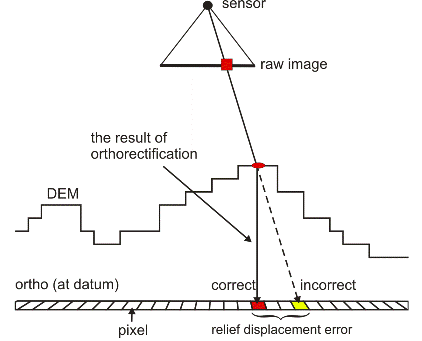
\includegraphics[width=0.6\textwidth]{figures/C2/Ortophoto.png}
    \caption{Orthorectification}
    \label{fig:orthorectification}
\end{figure}
The overall quality of the orthorectified image is therefore directly related to how accurate is the camera model and to the fidelity of the DEM. For this practical case the accuracy requirements of the georeferenced image is not so tight and so it has been decided, at first place, to use the ready-to-use Google Earth imagery database. Anyway in designing the mission work-flow it was predisposed the possibility to take an aerial photo of the entire site to georeference it.
% subsection ortho_rectification (end)

\subsection{Google Earth} % (fold)
\label{ssec:orthophoto_database}

\textit{"Google Earth is a virtual globe, map and geographical information program that was originally called Earth Viewer 3D, and was created by Keyhole, Inc, a Central Intelligence Agency (CIA) funded company acquired by Google in 2004. It maps the Earth by the superimposition of images obtained from satellite imagery, aerial photography and GIS 3D globe. Google Earth uses digital elevation model (DEM) data collected by NASA's Shuttle Radar Topography Mission (SRTM). The internal coordinate system of Google Earth is geographic coordinates (latitude/longitude) on the \acrfull{wgs84} datum i.e., the same datum that used by GPS."} \cite{PosAccuracyGE}.\\

Google Earth shows the earth surface as it looks from an elevated platform such as an airplane or orbiting satellite. The projection used to achieve this effect is called the General Perspective. This is similar to the Orthographic projection. Most of the high resolution imagery in Google Earth Maps is the Digital Globe Quickbird which is roughly 65cm pan sharpened. Google is actively replacing this base imagery with 2.5 m SPOT Image imagery and several higher resolution datasets.

The application is multi-platform and has an user friendly interface which among other provides tools to trace geographic feature such as shape, polygons and path. This turns out to be an essential feature in representing the field border which is after all, the final aim of this module. \todo{sinonimo di module???}.\\
The position accuracy of Google Earth was analyzed by Ahmed Ghazi whose selected 16 points in Khartoum
town. As of October 2012 The root mean square of the error results to be about $1.80m$ for horizontal position and $1.773m$ for height estimation.\cite{PosAccuracyGE} These results, while referring to only a specific region of the earth, are representative of the goodness of the data, especially considering they are available for free.\\
% subsection google_earth (end)
% section georeferenced_photo (end)

\section{Border Representation and Detection} % (fold)
\label{sec:border_detection_and_representation}
In order to obtain a digital representation of the border it is, first of all, important to define how to store the data in a file. Google Earth file format is the Keyhole Markup Language (KML).

\subsection{KML: Google Earth file format} % (fold)
\label{sub:kml_google_earth_file_format}
KML is an XML language focused on geographic visualization, including annotation of maps and images.
It became an international standard maintained by the Open Geospatial Consortium, Inc. (OGC).
KML can be used to:
\begin{itemize}
\item Annotate the Earth
\item Specify icons and labels to identify locations on the surface of the planet
\item Create different camera positions to define unique views for KML features
\item Define image overlays to attach to the ground or screen
\item Define styles to specify KML feature appearance
\item Write HTML descriptions of KML features, including hyperlinks and embedded images
\item Organize KML features into hierarchies
\item Locate and update retrieved KML documents from local or remote networklocations
\item Define the location and orientation of textured 3D objects
\end{itemize}

From a technical point of view, KML uses a tag-based structure based on XML standard \cite{bray06xml11}. All tags are case-sensitive and must be taken from the "KML Reference"\footnote{available at \url{https://developers.google.com/kml/documentation/kmlreference}}. \autoref{fig:KML-diagram} shows the most important attribute of a KML object. There are many object types, but for the application under interest some basic types like placemarks/points and lines are enough.
\begin{figure}[ht]
    \centering
    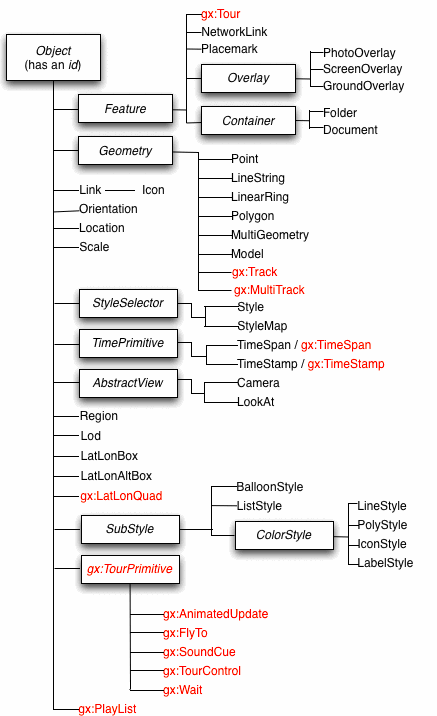
\includegraphics[width=0.5\textwidth]{figures/C2/KML-classTree.png}
    \caption{KML Object Hierarchy Diagram}
    \label{fig:KML-diagram}
\end{figure}

% subsection kml_google_earth_file_format (end)

\subsection{Field Border in KML} % (fold)
\label{sub:field_border_in_kml}
A border it is basically a close path having an undefined shape and therefore it cannot be represented using one polygon or other predefined geometric shapes. In KML such kind of geometric path should be defined through the object \textit{LineString}. LineString creates a path from a set of geographic points. Each adjacent point is connected with a line and finally if the ending point coincide with the starting one a close path is obtained. Clearly, this approach required an adequate number of points to make the resulting shape smooth. Fortunately, the generation of the points is automatically done by Google Earth which provides an handy toolbox to graphically create a path object directly drawing it over the map.
An example of a field contour encoded in KML code is reported in \autoref{list:border-KML}, where the complete list of coordinates has been omitted as it would be too long.

\lstinputlisting[label=list:border-KML, caption=Border in KML, language=XML]{listings/C2/border-valentino-field.kml}

Using the \textit{name} and \textit{description} tags gives the possibility to add meta-data to the KML geographic feature. This comes in handy to classify the field and creating a database of the place already visited. The idea is then to use the data already collected when repeating mission in a previously scanned field.
Before entering in the implementation details an example of how the contour appears in Google Earth is displayed in \autoref{fig:waldpeter-boundary-GE}.
\begin{figure}[ht]
    \centering
    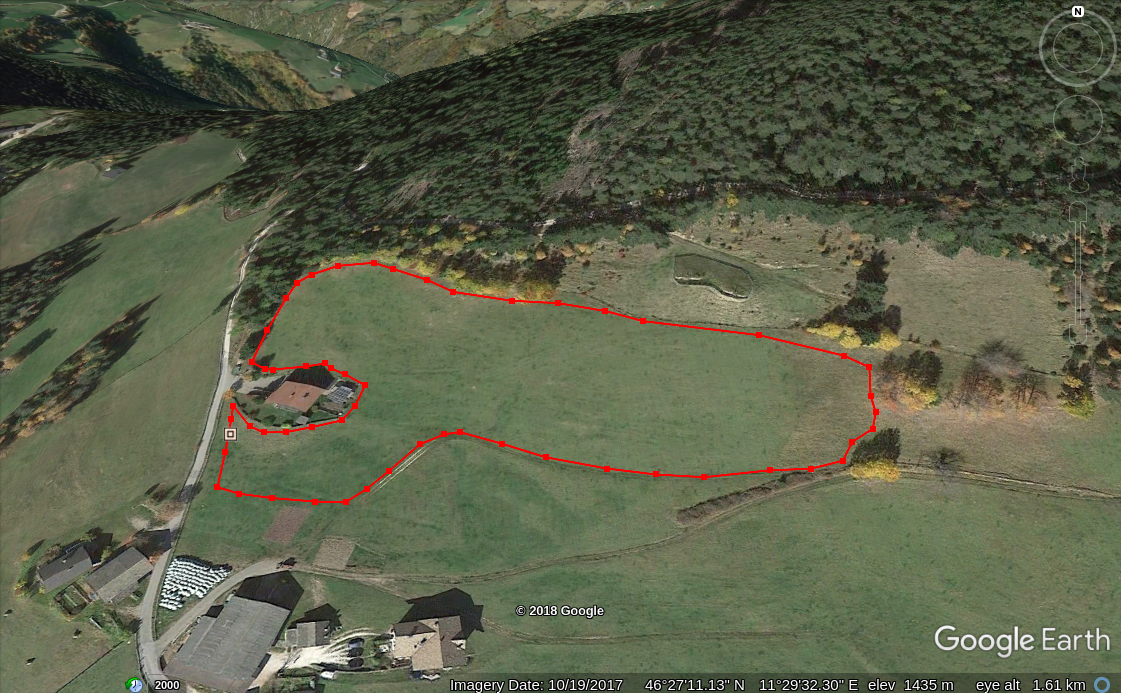
\includegraphics[width=0.9\textwidth]{figures/C2/waldpeter-boundary-GE.png}
    \caption{KML LineString geographic feature visualize on Google Earth}
    \label{fig:waldpeter-boundary-GE}
\end{figure}

\section{Implementation} % (fold)
\label{sec:implementation}
As it was accennato in \ref{sub:ortho_rectification} although the source of the orthophoto used in the software implementation is Google Earth, in defining the mission it has been taken into account the possibility to ??shut?? a photo of the whole field and georeference it (that is the goal of \textit{/optical\_cam} node). This would provide a ??more?? up-to-dated and eventually more accurate image, but at the same time the orthophoto generation is computationally heavy especially for a mini PC. This in addition to the limited flight time of the quadcopter suggest to use Google imagery database.
In the following section it is explained how this part of the mission has been implemented in \acrshort{ros}. The most relevant part concerns the representation of the field contour as \acrshort{ros} message and the way to import it given the respective KML file.

\subsection{ROS Nodes Architecture} % (fold)
\label{sub:ros_nodes}
\autoref{fig:field-detection-rqt} shows how the three \acrshort{ros} nodes (\textit{/mission\_controller},\textit{/optical\_cam} and \textit{/mission\_controller}, \textit{/boundary\_generator} and ), displayed as ovals, communicate together through the four topics represented inside rectangles. The node named \textit{/mavros} (for more details see appendix \ref{appendix:mavros}) on the left side of the diagram, manages everything regarding the communication with the aircraft. It basically provide a \acrshort{ros} interface to read the vehicle status variables and to change the flight controller behaviors.\par
\begin{figure}[ht]
    \centering
    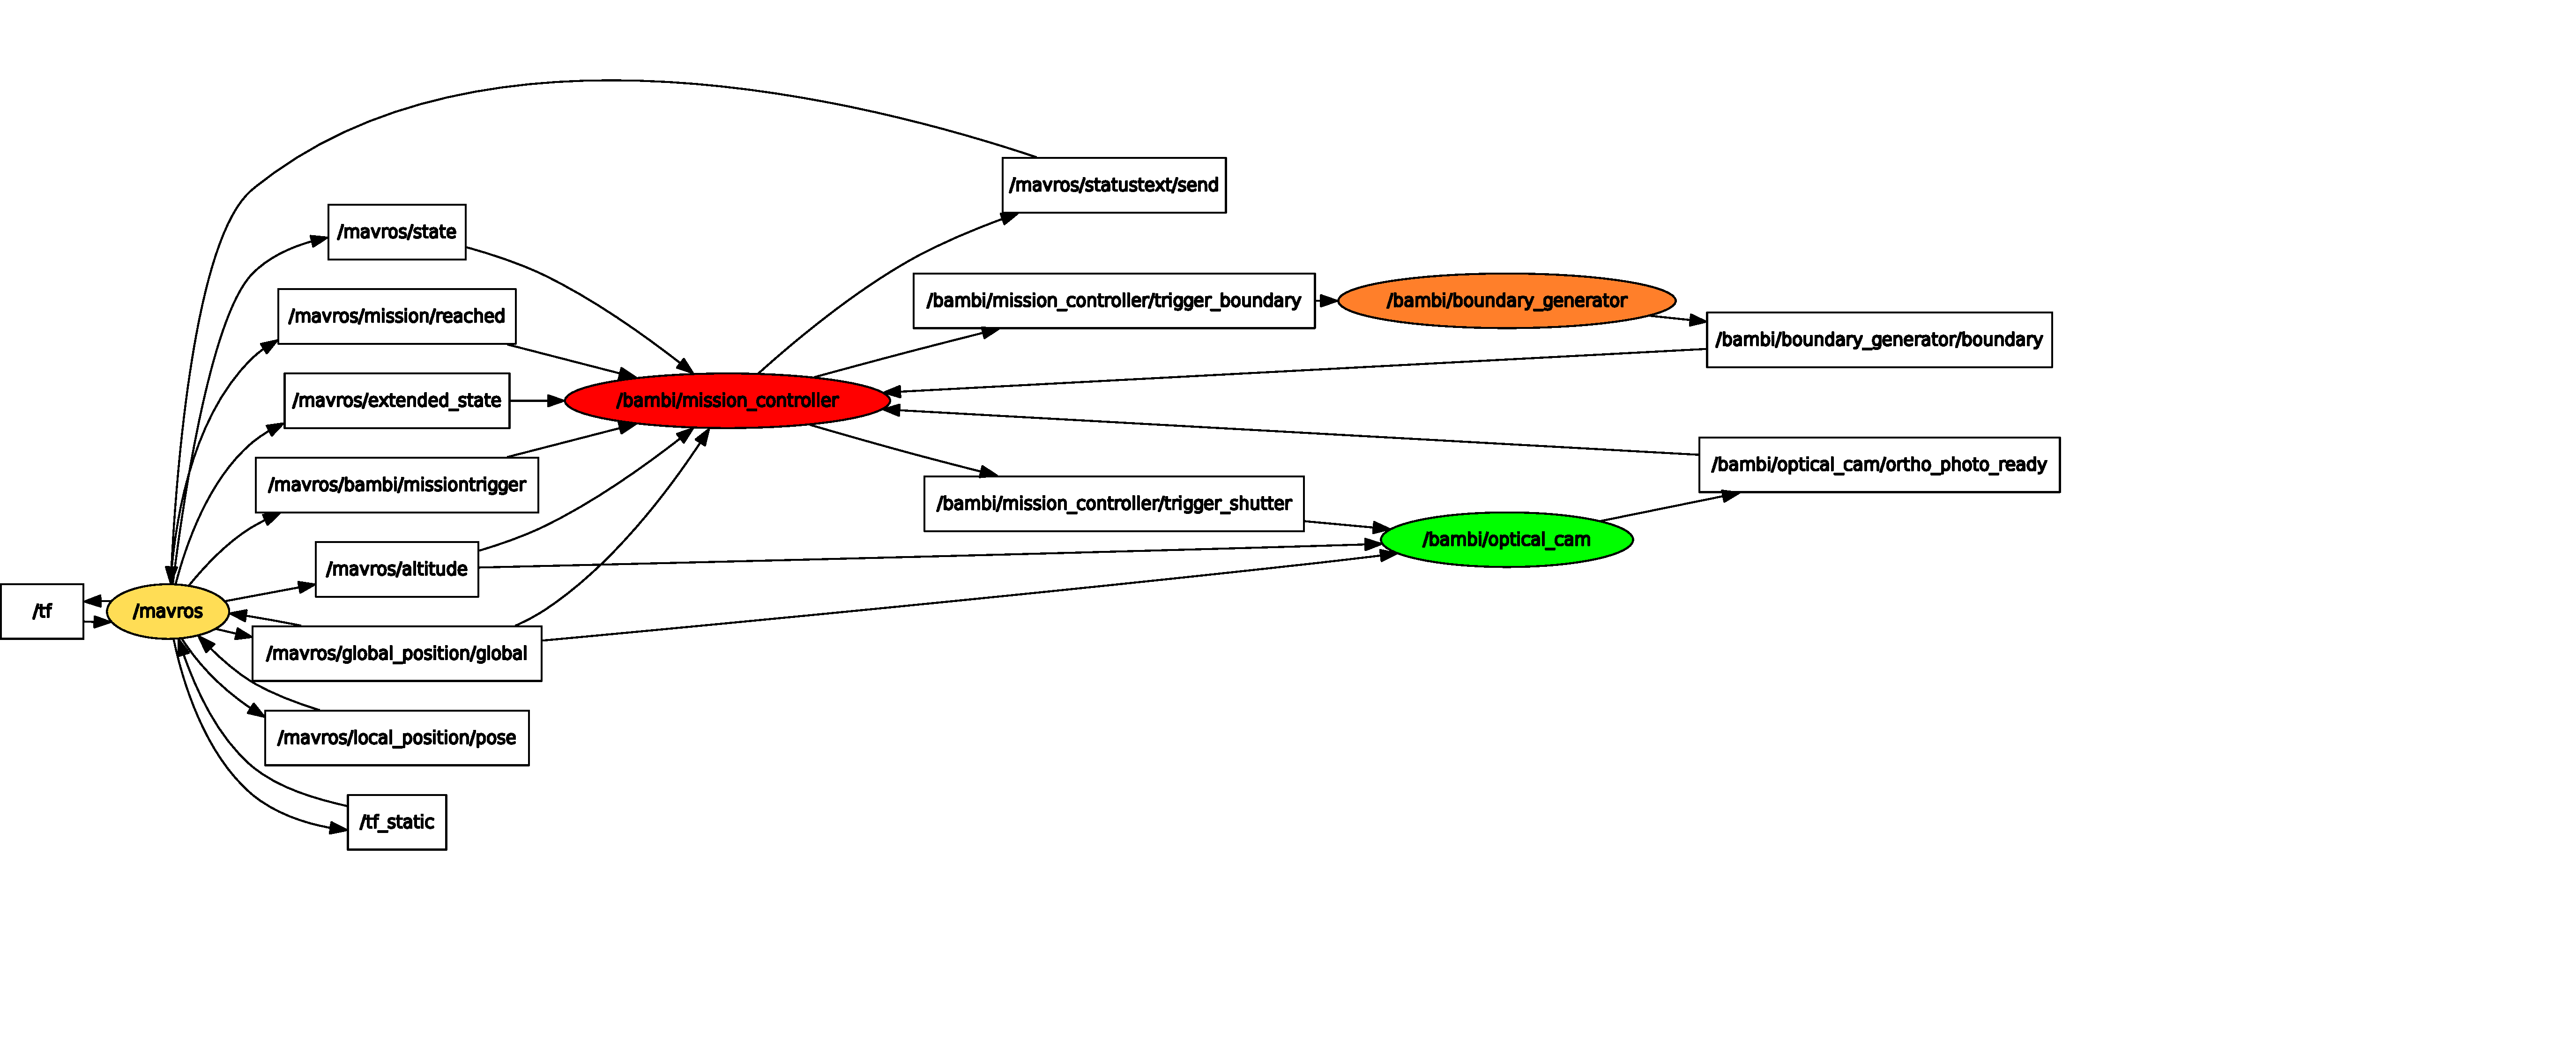
\includegraphics[width=1.3\textwidth]{figures/C2/fieldDetection-rqt_graph.pdf}
    \caption{Nodes and Topics concurring in generating the field contour}
    \label{fig:field-detection-rqt}
\end{figure}
Nodes specs:
\begin{itemize}
	\item \textit{/mission\_controller}: it is the node which contains the core of the mission. Through the implementation of a finite state machine it handle every mission steps and the transition among them. For what concern the scope of this chapter the main task of this node is to trigger the other two node, which really carry out the desired tasks.
	\item \textit{/optical\_cam}: upon the receiving (??reception??) of the \textit{trigger\_shutter} message from the mission controller node it triggers the camera shutter and saves the exact GPS position required to geo-tag the photo of the field.
	At this point the node, in case the it has been chosen to georeference the image locally, will generate the orthophoto. The orthophoto algorithm has not been implemented yet as explained at the beginning of this section.
	The node finish its job once it publishes the message containing the position of the orthophoto back to the \textit{/mission\_controller} node over the \textit{orthophoto\_ready} topic. 
	\item \textit{/boundary\_generator}: This node when triggered is suppose to elaborate the field boundary and sand it to the mission controller node. The communication happens through the two topics \textit{trigger\_boundary} and \textit{boundary} as shown in the nodes graph.
\end{itemize}
\subsubsection{Relevant message definitions} % (fold)
\label{ssub:relevant_message_definitions}
\textit{QUI INSERIRE LISTING DELLA DEFINIZIONE DEI MESSAGGI USATI DAI DUE NODI}

Now that a briefly introduction of each node has been done, a deeper analysis of the \textit{/optical\_cam} node and \textit{/boundary\_generator} node is carried out.
% subsubsection relevant_message_definitions (end)


\subsubsection{optical\_cam} % (fold)
\label{ssub:optical_cam}
This node has been written in python and it is responsible of the communication between the action camera (Xiaomi Yi Cam) and the other nodes running on the companion computer (raspberry Pi 3b). The camera communicate through WIFI in a server-client like fashion using the TCP protocol. For this reason, in python, the communication is managed using \textit{socket} library.
Once the socket is connected it is possible to send a several different command (in the form of \textit{token}) to remotely control the camera.\\
The first task of the node is to trigger the camera shutter when requested by the mission controller. The image is fetched and downloaded to the internal storage of the Raspberry, as soon as the camera sends back the message which tells it has successfully taken the photo. All this logic is implemented in the function \textit{take\_photo} listed in \autoref{list:camera_photo}. Most of the credits goes to Res Andy for its great effort in reverse engineering the Yi Cam remote control protocol and to provide sample scripts in python. \cite{YiCamGit}
Along with the trigger command, the node continuously listen to the topic \textit{/mavros/global\_position/global} where mavros node publishes the global position communicated by the flight controller (GPS fix). In this way the node has the necessary information to geo-tag the photo.
Once the photo is geotagged and made available locally on the onboard computer the \textit{optical\_cam} node would be in charge of generating the orthophoto. This part, at first place, has been omitted and ??leaved?? to future developments.
% \pagebreak
\lstinputlisting[label=list:camera_photo, caption=take\_photo() function in python, language=python]{listings/C2/camera_photo.py}
% subsubsection optical_cam (end)

\subsubsection{boundary\_generator} % (fold)
\label{ssub:boundary_generator}
As for \textit{/optical\_cam} node, python has been chosen as programming language because of the libraries available.
The \textit{/boundary\_generator}'s goal is, when requested, to publish \acrshort{ros} message ("Field.msg") over the topic \textit{boundary} containing the array of 2D coordinates representing the field contour.
In the following implementation the boundary information is taken from a KML file containing the geographic path manually generated through Google Earth. It has been decided to make a separated for this simple parsing task so that in future it will be ready to hold any image processing algorithm to autonomously extrapolate the field outline from the orthophoto.
The code of this node is integrally reported in \autoref{list:boundary_generator}.\\
First of all the node subscribes to \textit{/mission\_controller/trigger\_boundary} in such a way that upon the arrival of a trigger message the callback function \textit{cb\_boundary\_trigger} is called. The callback function get the absolute path of the KML file from the message attribute \textit{filenameWithFullPath}. Now it comes to play the pyKML library.\\
pyKML is a Python package for creating, parsing, manipulating, and validating KML documents \cite{pyKML}. It is based on the \textit{lxml.objectify} API \footnote{It aims to hide the usage of XML behind normal Python objects, sometimes referred to as data-binding. It allows you to use XML as if you were dealing with a normal Python object hierarchy.\cite{lxml}} which provides access to XML documents in python program. Once the file has been opened it is possible to access to KML child member in the way shown at line 23 \todo{assicurarsi si possa riferirsi cosi'}. At this point it is just a matter of parsing each geographic point as it was a string in the form "<latitude>, <longitude>" using the function \textit{split(',')}.
Latitude and longitude coordinate for each point of the contour is then packed in a geoPosition2D object which is push back on the boudary\_path vector. Once every point has been parsed and the vector filled the \textit{Field} \acrshort{ros} message is published completing the node's job.
\lstinputlisting[label=list:boundary_generator, caption=boundary generator
 node in python, language=python]{listings/C2/boundary_generator.py}.

% subsubsection boundary_generator (end)

% subsubsection ros_nodes (end)

% because there is not an explanation for explain this. I have tryed to explained the most safe way to preserve the deers but the problem is all that I am not capable to explain what is happening in to myself . i trust of myself but one part of my think about the life it is not so much easy for think that i am really capable to talk about something. so finally i think that i must stop
%  my self to try to find some origins about something when I am not capable to talk about me, this thesis is another why to try to discover  about something that it is outward rather than something that are inside me. most of people are used to talk about different things around the world because for every man it is easier to talk about something that no concern about it self. they were more years that the most part of people thinks only about everything that concerns the world outside. the fact is that it is so difficult talk about himself. this is the reason why everybody tryes to write a test that no concern about himself. il fatto è mike che studiando tutto cio mche compete il mondo tu inevitabilmente perderai parte di te stesso. come evitare cio ricorda in ogni cosa di fermarti, respirare, e sentire te stesso. annusati come faresti con un profumo nuovo. comprendi ogni cellula di te stesso per comprendere cio che ami e vuoi. e così avverra che in ogni cosa in cui ti dedicherai ilcentro non sara perdibile poiche sara sempre la parte di te che in quel momento deciderai di far uscire, esprimere e essere.

% subsection field_border_in_kml (end)




% section border_detection_and_representation (end)

 